\section{Data}
\label{ckdata}

The data include -- with a few exceptions detailed below -- all roll-call votes in the U.S. House of Representatives during the 46th through 106th Congresses, corresponding to the period from 1879 to 2001.  Following Cox and Katz, excluded from the analysis are any records that meet at least one of the following three conditions: ({\it i}) the majority of both parties voted for the same position; ({\it ii}) the purpose of the vote was electing the Speaker of the House; ({\it iii}) the vote required a two-thirds majority for passage.

The resulting data consist only of votes that required a simple majority for passage and on which the Republican and Democratic parties were in clear opposition.\footnote{A brief comment on notation: for greater consistency throughout this paper, this section uses different notation than \citeA{cox_gerrymandering_2007}.}

Let $RC_{it}$ denote the result of roll-call vote $i$ in Congress $t$ such that 

\begin{equation*}
RC_{it} =
\begin{cases} 
1, & \text{ if Democratic position wins vote $i$ in Congress $t$,} \\[10pt]
0, & \text{ if Republican position wins vote $i$ in Congress $t$.}
\end{cases}
\end{equation*}
~\\[-12pt]

%\noindent Here, the Democratic position refers to the outcome preferred by the majority of Democrats.  The definition is analogous for the Republican position.

%The outcomes of interest are the number of wins ($w_t^{DEM}$) and proportion of wins ($\pi_t^{DEM}$) for the Democratic position in each Congress $t$
%
%$$ w_t^{DEM} = \sum_{i=1}^{n_t} RC_{it}, \qquad \pi_t^{DEM} = w_t^{DEM} / n_t.\footnote{The superscript {\it MAJ} (e.g. $y_t$) will be used later in the thesis as a general way of referring to the majority party in a specific time period. While the data is organized and more naturally described in terms of $w_t^{DEM}$ and $w_t^{REP}$ (which is just $n_t-w_t^{DEM}$), the proposed statistical model is more straightforward to implement in terms of $w_t^{MAJ.}$}$$
%
%Here $n_t$ is the number of roll-call votes in Congress $t$, which ranges from a minimum of 33 votes in the 70th Congress (1927-1929) to a maximum of 836 votes in the 104th Congress (1995-1997). The median number is 143 votes.  
%
%
%The sole predictor of interest is $v^{RATIO}$, the ratio of the average vote share earned by the Democratic position to the average vote share earned by the Republican position in each Congress.  For each Congress the average is taken over all roll-call votes.  For vote $i$ in Congress $t$, let $\pi_{it}^{DEM}$ be the proportion of representatives who cast their vote in favor of the Democratic position.  Then the mean vote shares for the Democratic and Republican positions in Congress t is
%
%{\singlespacing
%$$v_t^{DEM} = \frac{1}{n_t} \sum_{i=1}^{n_t} \pi_{it}^{DEM}, \qquad v_t^{REP} = 1 - v_t^{DEM}$$
%}
%%
%\noindent and the ratio of Democratic to Republican vote shares is simply $v_t^{RATIO} = v_t^{DEM} / v_t^{REP}$. Figure~\ref{fig:log_vratio_vs_ptdem} shows $\log{(v^{RATIO} )}$ plotted against $\pi^{DEM}$. The shape of the curve is similar to the standard seats-votes curve used in analyses of bias and responsiveness in electoral contexts. The curve is analogous in the legislative context of Cox and Katz's example, although we are not concerned with seat shares in a given Congress but rather roll-call vote shares ($\pi_t^{DEM}$ and $\pi_t^{REP}$). This is discussed further in the Methods section. 
%
%The trends of $\log{(v^{RATIO} )}$ and $\pi^{DEM}$ over time are shown in the visual summary of the data set in Figure~\ref{fig:data_summary}.
%
%%FIGURE
%\begin{figure}
%\centering
%	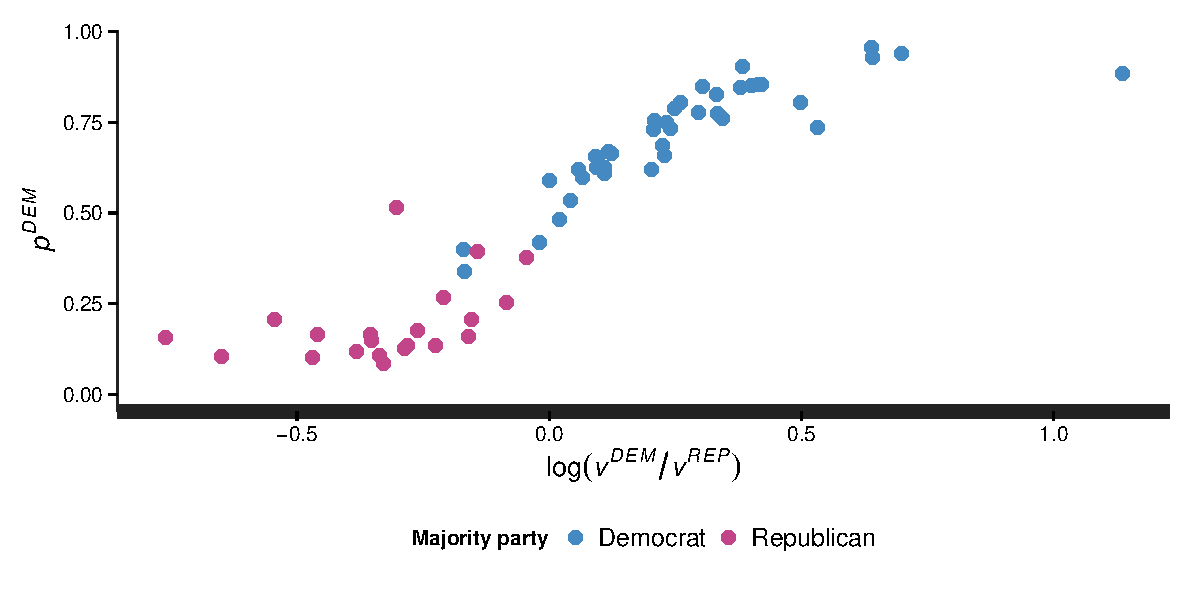
\includegraphics[scale=0.75]{sections/figs/logvratio_vs_pdem}
%\caption{$\log{(v^{RATIO} )}$  vs. $\pi^{DEM}$}
%\label{fig:log_vratio_vs_ptdem}
%\end{figure}
%%
%



\noindent The outcomes of interest are the number of wins $y_t$ and proportion of wins $\pi_t$ for the majority party position in each Congress $t$,

\begin{equation*}
y_t =
\begin{cases} \sum_{i=1}^{n_t} RC_{it}, & \text{ if Democrats hold majority}, \\[10pt]
n_t - \sum_{i=1}^{n_t} RC_{it}, & \text{ if Republicans hold majority,} \\
\end{cases}
\end{equation*}
~\\[-12pt]
 
\noindent and $\pi_t = y_t / n_t$. Here $n_t$ denotes the number of roll-call votes in Congress $t$.\footnote{The value of $n_t$ ranges from a minimum of 33 votes in the 70th Congress (1927-1929) to a maximum of 836 votes in the 104th Congress (1995-1997). The median number is 143 votes. See also Figure~\ref{fig:data_summary} (p. \pageref{fig:data_summary}).} 

The sole predictor is the ratio of the average vote share earned by the majority party position to the average vote share earned by the minority party position in each Congress.  (For each Congress the average is taken over all roll-call votes.)  For vote $i$ in Congress $t$, let $p_{it}^{DEM}$ be the proportion of representatives who cast their vote in favor of the Democratic position.  Then the mean vote shares for the Democratic and Republican positions in Congress t are

\begin{equation*}
v_t^{DEM} = n_t^{-1} \sum_{i=1}^{n_t} p_{it}^{DEM}, \qquad v_t^{REP} = 1 - v_t^{DEM},
\end{equation*}

\noindent and the ratio of Democratic to Republican vote shares is simply $v_t^{DEM} / v_t^{REP}$. The notation $v_t^{RATIO}$ will be used as shorthand for the ratio $v_t^{MAJ} / v_t^{MIN}$, that is 

\begin{equation*}
v^{RATIO} = 
\begin{cases} 
v^{DEM} / v^{REP}, & \text{ if Democrats hold the majority,} \\[10pt]
v^{REP} / v^{DEM}, & \text{ if Republicans hold the majority.} \\
\end{cases}
\end{equation*}
~\\[-12pt]


%FIGURE
\begin{figure}
\centering
	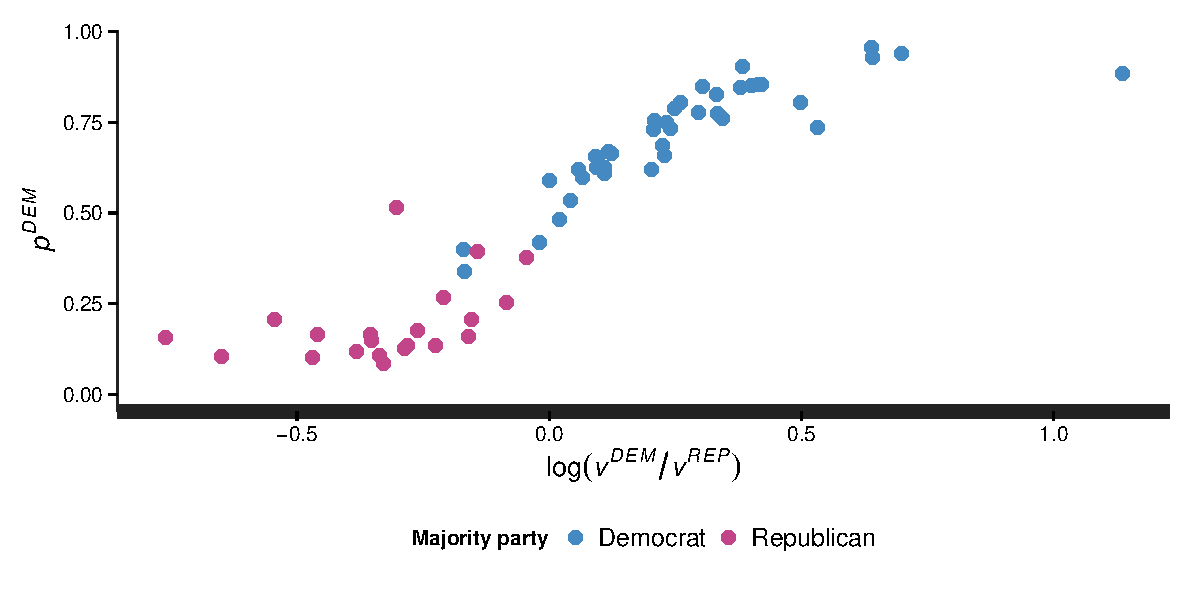
\includegraphics[scale=0.75]{sections/figs/logvratio_vs_pdem}
\caption{$\log{(v_t^{DEM} / v_t^{REP} )}$  vs. $\pi^{DEM}$}
\label{fig:log_vratio_vs_ptdem}
\end{figure}

Figure~\ref{fig:log_vratio_vs_ptdem} shows $\log{(v^{DEM} / v^{REP} )}$ plotted against $\pi^{DEM}$. The shape of the curve is similar to the standard seats-votes curve  

\begin{equation*}
 \frac{s}{1-s} = \exp{(\lambda)}\left(\frac{v}{1-v}\right)^\rho 
\end{equation*}

\noindent used in analyses of bias and responsiveness in electoral contexts. The curve is analogous in the legislative context of Cox and Katz's example, although we are not concerned with seat shares $s$ but rather roll-call vote shares $\pi$. This is discussed further in section \ref{subsection_methods} in relation to the statistical model. 

The trends of $\log{(v^{DEM} / v^{REP} )}$ and $\pi^{DEM}$ over time are shown in the visual summary of the data set in Figure~\ref{fig:data_summary}.


%FIGURE
\begin{figure}[p]
\centering
	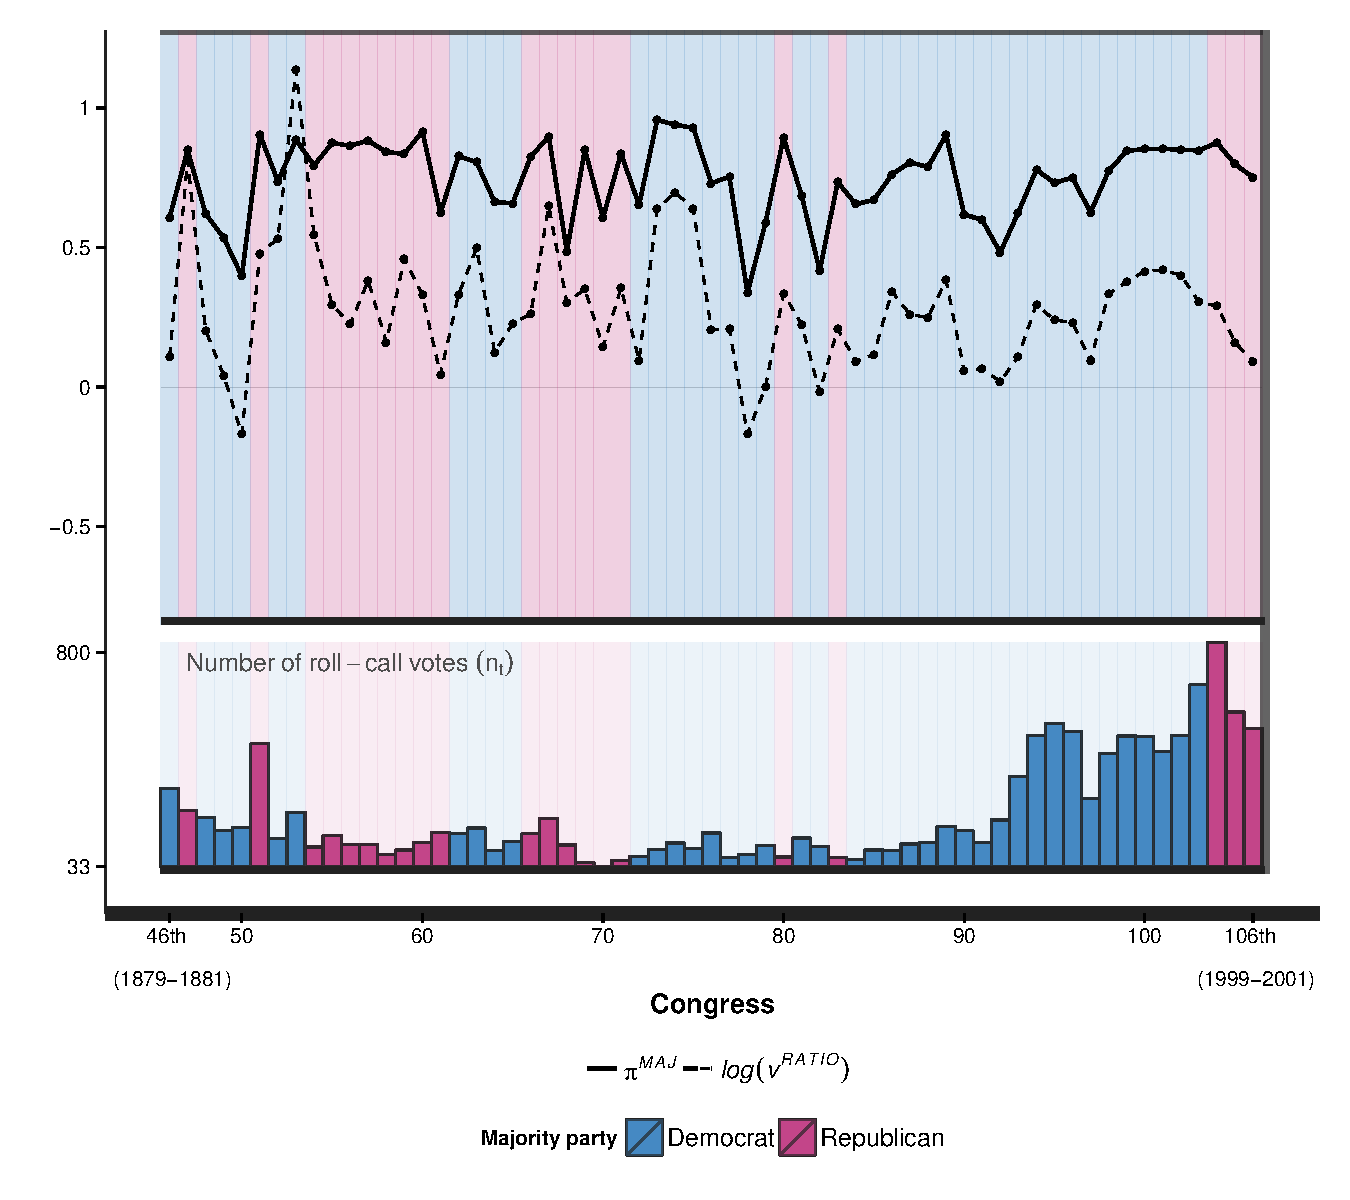
\includegraphics[scale=0.75]{sections/figs/vis_summary}
\caption{Visual summary of the data. The trends of $\log{(v_t^{DEM} / v_t^{REP} )}$ and $\pi^{DEM}$ by Congress are plotted on top, with the number of roll-call votes per Congress below. Background shading is used to differentiate between Democratic and Republican majorities.}
\label{fig:data_summary}
\end{figure}
%

%One method of identifying bias toward or against the majority party is to estimate $E[p_t |v_t^{MAJ}=0.5]$, the proportion of majority party victories conditional on equal vote share, and compare the estimate to $0.5$, the expected proportion of majority party victories in the absence of bias.  There are many close votes in the data -- that is, votes where $v_t^{MAJ} \approx 0$ -- which can be used to estimate $E[p_t |v_t^{MAJ}=0.5]$.  Figure 2, below, shows the proportion of majority party victories under four different definitions of a close votes corresponding to margins of victory of 0.125\%, 0.25\%, 0.5\%, and 1.0\%. 
%
%\vskip1cm
%FIGURE
%\vskip1cm

